\section{Methodology details}
\label{supsec:methods-detail}



\paragraph{Architecture of our network. }
\label{methods:network-arch-detail}
The schematic depiction of our architecture is in Figure~\ref{fig:architecture}. Note that the architecture of the model varies slightly depending on the task (eg, on the number of predicted categories). 


\begin{figure}[!t]
\label{fig:architecture}
\centering
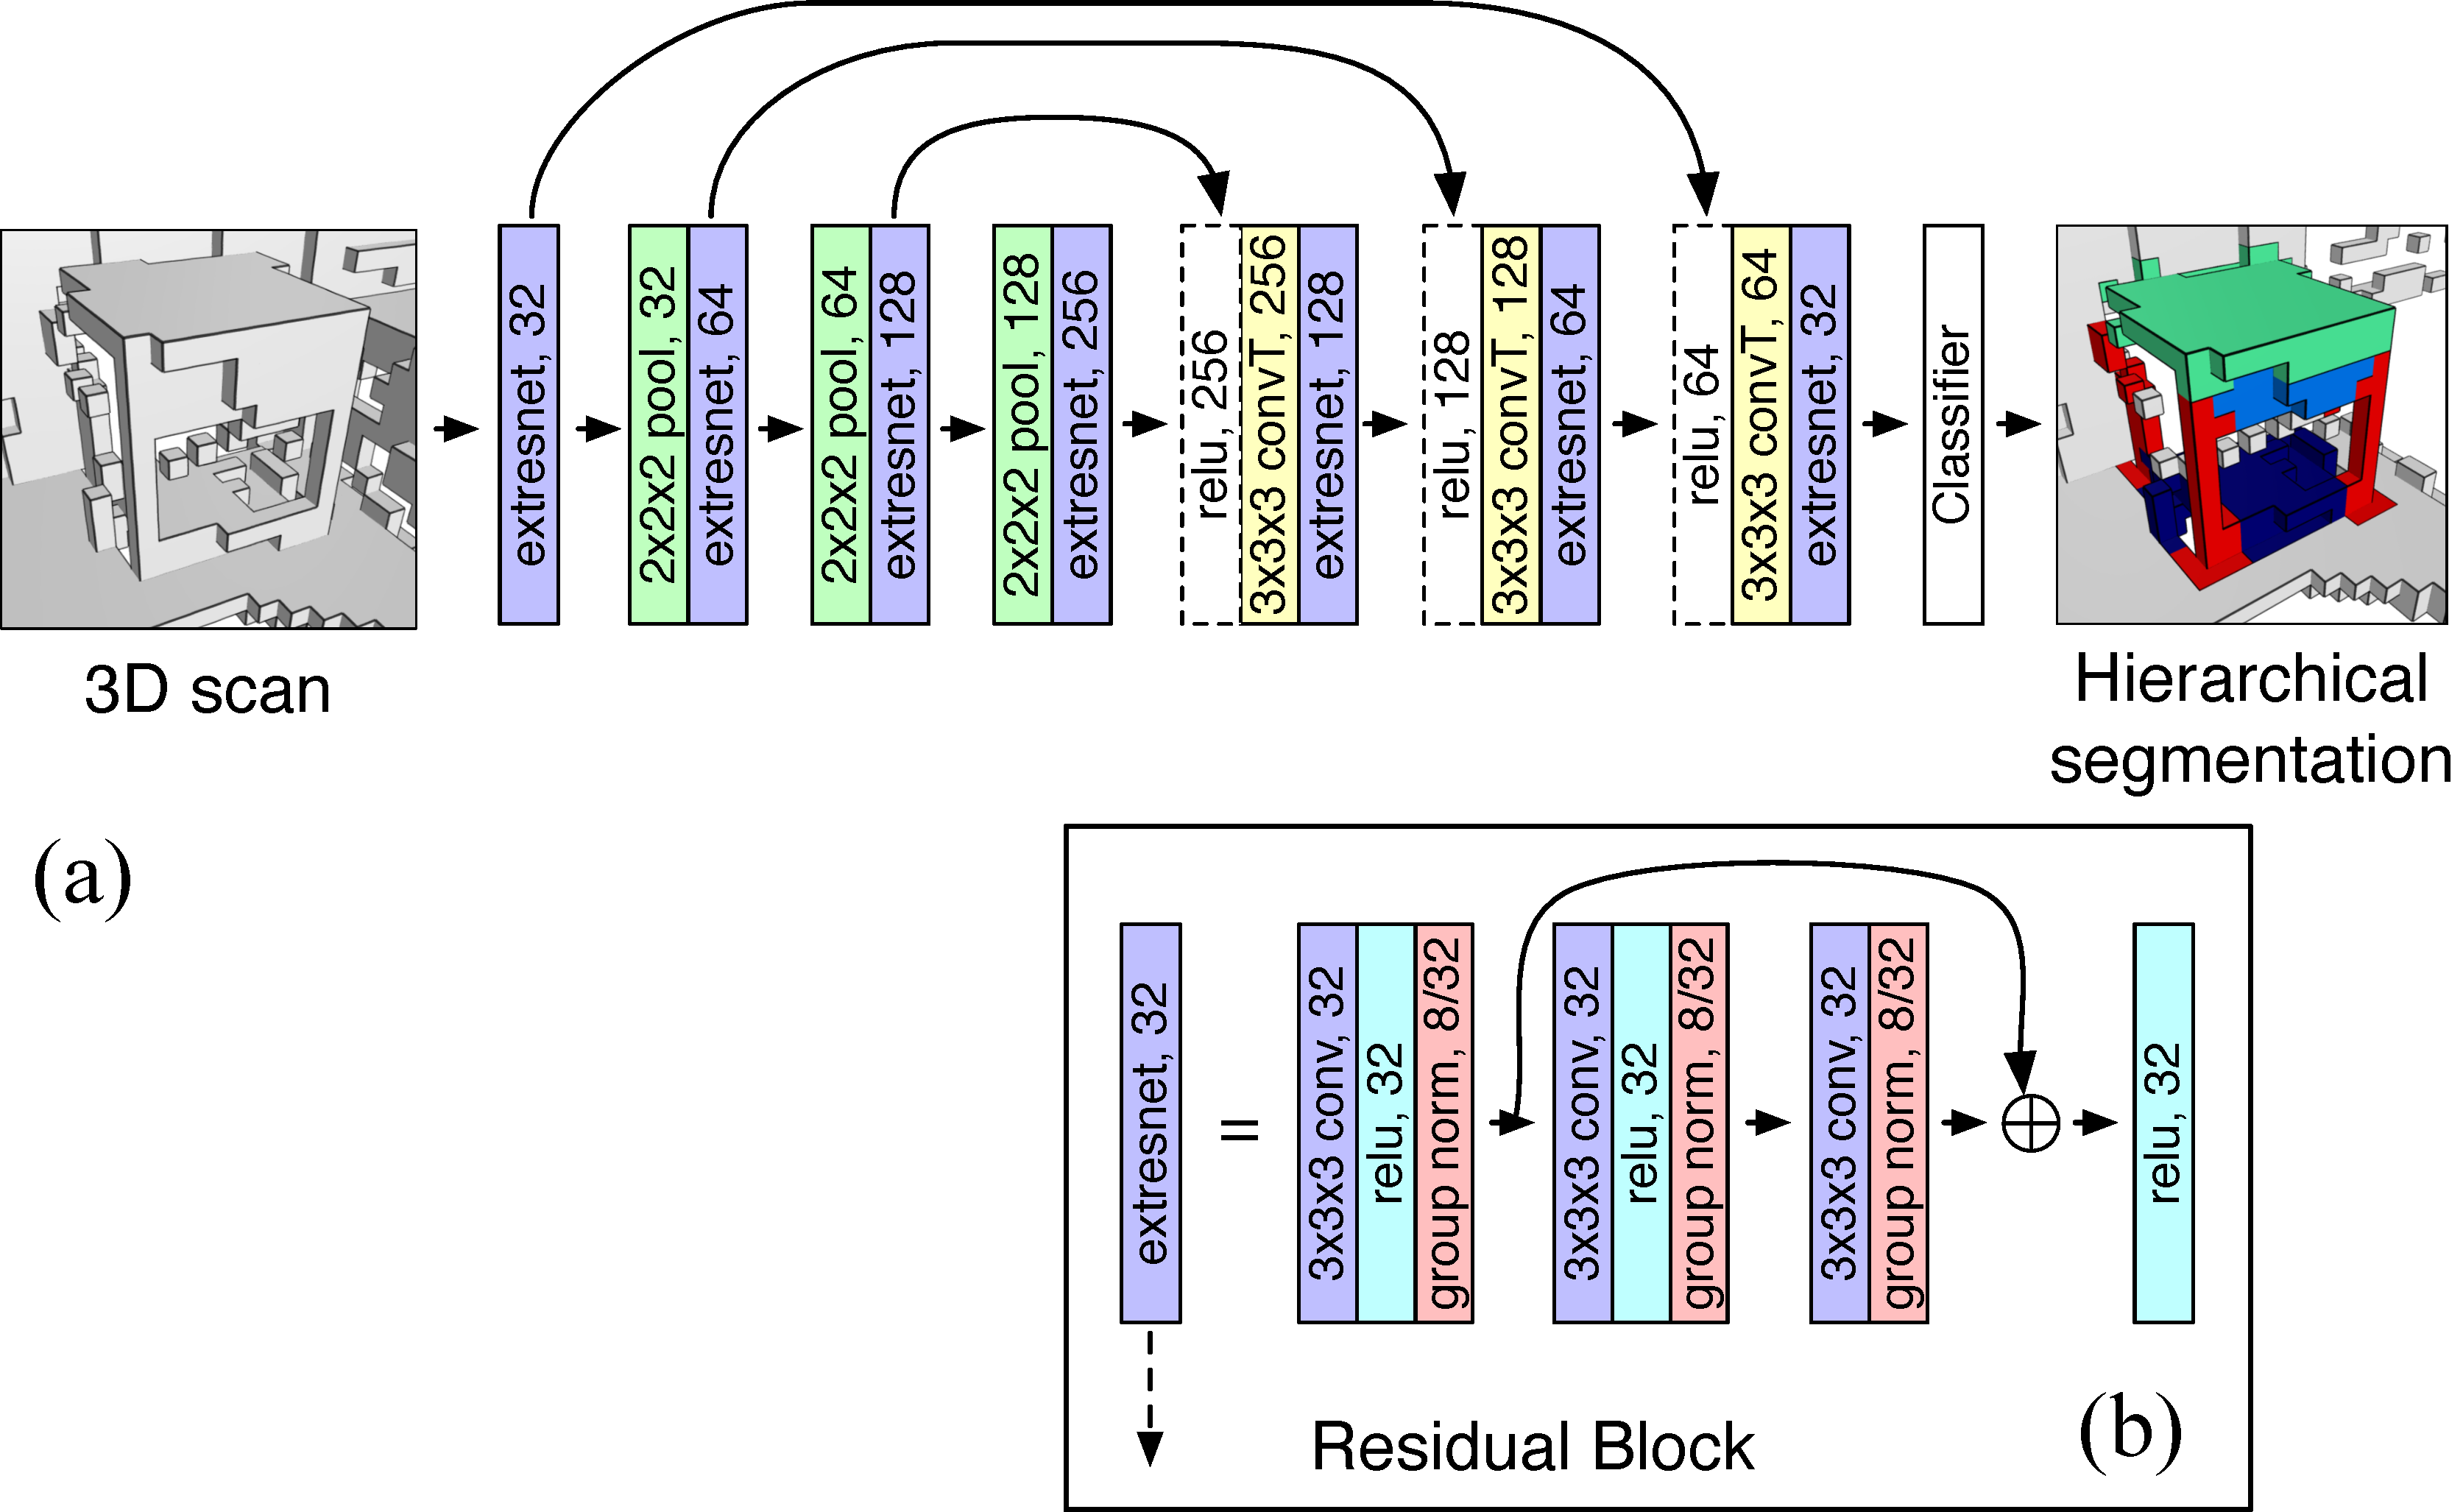
\includegraphics[width=0.9\textwidth]{images/scannet-unet3d-model-architecture}
\caption{The architecture of our model. Our architecture is a 3D U-net with residual blocks equipped with ReLU non-linearities and groupwise normalization layers. The model has 4 encoder and 3 decoder blocks with upsampling performed by transposed convolutions.}
\end{figure}



% \LA{figure displaying the architecture}


%  • [189] Specifically, as a backbone for our models we use a 3D version of the U-net architecture [57] with residual modules in both encoder and decoder branches (based on [58, 59]; see supplementary for a full network architecture) — здесь у нас есть картинка структуры сети, нужно ли что-то добавлять?

%  3. Визуализации архитектур, детальные для всех случаев. картинка структуры сети (есть одна из трёх) (отсылка к строке 189 основной статьи) 



\paragraph{Loss function for semantic instance segmentation. }
\label{methods:loss-detail}

To perform efficient voxel-wise instance segmentation, we opt to learn \emph{voxel embeddings} akin to \emph{pixel embeddings} in~\cite{de2017semantic}, aiming to cluster embeddings for the same object part together while pushing embeddings for separate parts farther apart.
To this end, we employ a multi-task loss function given by:
\begin{equation}
\label{eq:ours_instance_seg_loss}
L = \alpha_{\text{intra}} L_{\text{intra}}
  + \alpha_{\text{inter}} L_{\text{inter}}
  + \alpha_{\text{reg}} L_{\text{reg}}
  + \alpha_{\text{sep}} L_{\text{sep}}
\end{equation}
where 
$L_{\text{intra}}$ is an intra-part term aiming to pull embeddings of voxels with the same part ID closer together,
$L_{\text{inter}}$ is an inter-cluster term, pushing \emph{mean} voxel embeddings with distinct part IDs farther apart from each other,
$L_{\text{reg}}$ keeps the network activations bounded, thus acting as a regulartization term, and
$L_{\text{sep}}$ aims to enforce separation between objects and background representations in feature space. 
Constants $\alpha_{\text{intra}}, \alpha_{\text{inter}}$ are set to 1, and $\alpha_{\text{reg}}, \alpha_{\text{sep}}$ are set to 1e-3 in our evaluation. We evaluated Instance Segmentation with $L_{\text{sep}}$ only on coarse level of detail.
While the first three terms are identical to those in~\cite{de2017semantic,pham2019jsis3d}, the separation term $L_{\text{sep}}$ may be written down as:
\begin{equation}
\label{eq:ours_instance_seg_loss_sep_term}
L_{\text{sep}} = [\max_i|\mathbf{x}^{\text{fg}}_i - \mu|_1 - |\mathbf{x}^{\text{bg}}_i - \mu|_1 + \delta]_+
\end{equation}
where $\mathbf{x}^{\text{fg}}_i$ and $\mathbf{x}^{\text{bg}}_i$ are voxel embeddings for the part and background voxels, respectively, $\mu = \frac 1 N \sum_i \mathbf{x}^{\text{fg}}_i$ is the mean embedding for foreground voxels, and $\delta > 0$ is a hyper-parameter specifying the margin where the foreground-background separation force is active.








